% LaTeX support: latex@mdpi.com
\documentclass[investment,article,submit,pdftex,moreauthors]{Definitions/mdpi}

\firstpage{1}
\makeatletter
\setcounter{page}{\@firstpage}
\makeatother
\pubvolume{1}
\issuenum{1}
\articlenumber{0}
\pubyear{2026}
\copyrightyear{2026}
\externaleditor{}
\datereceived{}
\daterevised{}
\dateaccepted{}
\datepublished{}

\usepackage{amsmath}
\usepackage{mathtools}
\usepackage{graphicx}
\usepackage{booktabs}
\usepackage{array}
\usepackage{caption}
\usepackage{subcaption}
\usepackage{float}

\Title{Validating ETF Proxies for Fama French Style Factors: Evidence from Classification Based Trading Strategies}

\newcommand{\orcidauthorA}{0000-0000-0000-0000}
\newcommand{\orcidauthorB}{0000-0002-3836-1851}

\Author{Shivam Bhardwaj$^{1}$\orcidA{} and Eugene Pinsky$^{2,*}$\orcidB{}}

\address{%
$^{1}$ YRISE, Yale University; shivamb@bu.edu \\
$^{2}$ Department of Computer Science, Metropolitan College, Boston University, 1010 Commonwealth Avenue, Boston, MA 02215, USA; epinsky@bu.edu}

\corres{Correspondence: epinsky@bu.edu}

\abstract{Academic factor returns are central to empirical asset pricing, but the characteristic sorted portfolios used to construct them are not directly traded by most investors. This paper studies whether liquid exchange traded funds can serve as tradable proxies for Fama French style size, value, profitability, and investment factors. Proxy definitions are selected and evaluated using factor replication criteria rather than trading performance. The analysis first validates each ETF spread against the corresponding official factor return using correlation, sign agreement, tracking error, and single proxy regressions. It then evaluates whether simple allocation rules can improve the choice between the two ETF legs of each proxy. The strategies include a Winners and Losers rule, a nearest neighbor classifier, and logistic regression, all estimated with expanding windows and evaluated net of transaction costs. The results show that proxy quality is a first order determinant of interpretation. The size proxy closely tracks SMB, the value proxy provides a meaningful approximation to HML, and the profitability and investment proxies provide more moderate empirical approximations. In the trading tests, no method dominates across all factors and frequencies. Weekly KNN substantially reduces turnover relative to daily KNN while preserving or improving Sharpe ratios for several proxies. Logistic regression is most competitive for the value proxy, where a simpler and more interpretable classifier outperforms the more flexible nearest neighbor rule. The evidence supports a cautious view of ETF based factor timing: classification methods can add value in selected cases, but their interpretation depends critically on proxy validity, trading frequency, and implementation costs.}

\keyword{factor models; exchange traded funds; Fama French factors; KNN; logistic regression; trading strategies; transaction costs}

\begin{document}

\section{Introduction}

Factor models are central to modern empirical asset pricing and portfolio construction. The work of \citet{fama1993common} shows that equity returns contain common variation related to the market, firm size, and book to market characteristics. \citet{fama2015five} extend this framework by adding profitability and investment factors, producing the five factor model now widely used for performance evaluation, risk attribution, and the study of cross sectional return premia.

The empirical importance of these factors does not make them directly investable. Fama and French factor returns are constructed from diversified long short portfolios sorted on firm characteristics, while most investors obtain style exposures through listed securities or exchange traded funds. This creates a practical gap between academic factor definitions and portfolios that can be traded without building characteristic sorted stock portfolios. This paper studies that gap by asking whether ETF based return spreads can serve as tradable proxies for the non market components of the Fama and French five factor model.

The analysis focuses on four factor proxies: size, value, profitability, and investment. Each proxy is constructed as the return difference between two liquid ETFs chosen to represent opposite economic exposures. The size proxy compares small capitalization equities with broad large capitalization equities. The value proxy compares value stocks with growth stocks. The profitability proxy compares quality oriented stocks with speculative innovation oriented stocks. The investment proxy compares high quality conservative firms with Nasdaq growth exposure. Before any trading strategy is evaluated, the paper tests whether these ETF spreads explain the corresponding official Fama and French factor returns.

This validation step is essential. A strategy based on a weak proxy may generate performance that reflects ETF specific behavior rather than exposure to the intended academic factor. The paper therefore separates the factor replication problem from the timing problem. First, official factor returns are regressed on ETF proxy returns. Second, the proxy legs are treated as an implementable allocation problem in which the investor chooses one ETF leg at each decision date.

The trading exercise compares three allocation approaches. The first is a rule based Winners and Losers strategy motivated by the literature on return continuation and reversal \citep{debondt1985overreact,jegadeesh1993returns}. The second is a nearest neighbor classifier that uses historical return and volatility patterns to identify similar past observations. The third is logistic regression, which estimates the probability that one ETF leg will outperform the other in the next period. These methods are intentionally simple. Their purpose is not to exhaust the machine learning toolkit, but to test whether modest classification structure adds value once the factor proxy is made tradable.

The paper contributes to the literature in three ways. First, it provides direct evidence on how well liquid ETF pairs replicate official Fama and French factors. Second, it compares rule based and classification based allocation methods within the same tradable proxy framework. Third, it evaluates the results under realistic implementation assumptions, including daily and weekly trading frequencies and proportional transaction costs. This matters because trading frictions can materially affect the profitability of anomaly based strategies \citep{frazzini2014trading}.

The evidence shows substantial heterogeneity. The size proxy has strong explanatory power for the official SMB factor, while the value proxy explains a meaningful share of HML variation. The profitability and investment proxies provide more moderate explanatory power. Strategy performance is also uneven across factors and trading frequencies. This heterogeneity is the main empirical message of the paper. Tradable factor timing depends not only on the forecasting rule, but also on the quality of the ETF proxy being traded.

The remainder of the paper is organized as follows. Section 2 reviews related literature. Section 3 describes the data, ETF proxy construction, validation regressions, trading rules, and performance measures. Section 4 reports the empirical results. Section 5 discusses robustness and interpretation. Section 6 concludes.

\section{Related Literature}

This paper relates to three strands of literature: empirical asset pricing factor models, tradable factor implementation, and classification based trading strategies.

The first strand is the literature on factor models and return premia. \citet{fama1993common} establish the three factor model, showing that size and book to market factors help explain common variation in stock returns beyond the market factor. \citet{fama2015five} extend the framework by adding profitability and investment factors. Their model is motivated by valuation theory and captures empirical patterns in which firms with higher profitability and more conservative investment tend to earn higher average returns. Related work by \citet{novymarx2013other} shows that profitability is a powerful predictor of average returns and provides an important foundation for the profitability dimension of the five factor model.

The second strand studies implementation. Academic factors are usually constructed from broad long short portfolios, but ETFs offer liquid and transparent vehicles for accessing style exposures. ETF returns may, however, differ from the academic factors they are intended to represent. \citet{bendavid2017exchange} discuss the growth of ETFs and their role in liquidity, price discovery, and market structure. \citet{petajisto2017inefficiencies} shows that ETF prices can deviate from underlying net asset values, which reinforces the need to treat ETF implementation as an empirical question rather than a mechanical translation of academic factors.

The third strand concerns return predictability and statistical learning. \citet{debondt1985overreact} document evidence consistent with long horizon reversals, while \citet{jegadeesh1993returns} show that intermediate horizon winner portfolios outperform loser portfolios. These results motivate the use of recent relative performance as a signal, but they also show that the sign and horizon of predictability matter. \citet{lo2000foundations} provide a statistical treatment of technical analysis and show how historical price patterns can be evaluated systematically. More recently, \citet{gu2020empirical} demonstrate that machine learning methods can improve empirical asset pricing forecasts by capturing nonlinearities and interactions that are difficult to model with standard linear specifications.

This paper sits at the intersection of these literatures. It does not treat Fama and French factors as traded assets. It first constructs ETF based proxies and tests whether they track the intended academic factors. It then studies whether simple classification methods can improve allocation between the two ETF legs of each proxy.

\section{Data and Methodology}

\subsection{Data and ETF Proxy Construction}

The study uses daily Fama and French five factor returns and daily ETF returns. The Fama and French data consist of the excess market factor \((MKT\text{-}RF)\), small minus big \((SMB)\), high minus low \((HML)\), robust minus weak \((RMW)\), conservative minus aggressive \((CMA)\), and the risk free rate \((RF)\). These series are obtained from the Kenneth R. French Data Library \citep{frenchdatalibrary}.

ETF returns are computed from adjusted closing prices so that dividends and splits are reflected in the return series. ETF expense ratios are reflected in fund net asset value performance and therefore enter the adjusted price return series indirectly. The market benchmark is represented by SPY. The ETF proxy definitions are
\begin{align}
SMB^{ETF}_{t} &= r_{IJR,t} - r_{SPY,t}, \\
HML^{ETF}_{t} &= r_{SPYV,t} - r_{SPYG,t}, \\
RMW^{ETF}_{t} &= r_{QUAL,t} - r_{ARKK,t}, \\
CMA^{ETF}_{t} &= r_{SPHQ,t} - r_{QQQ,t}.
\end{align}

IJR represents small capitalization equities, SPY represents broad large capitalization U.S. equities, SPYV represents value stocks, SPYG represents growth stocks, QUAL represents quality stocks, ARKK represents speculative innovation oriented growth stocks, SPHQ represents S&P 500 quality stocks, and QQQ represents Nasdaq 100 growth oriented equities. The sample is restricted to the period in which all ETF legs are available, from 3 November 2014 to 30 April 2026.

The RMW and CMA ETF definitions require additional care because they do not have one to one ETF analogues. The RMW proxy is best interpreted as quality minus speculative innovation. The CMA proxy is best interpreted as quality and conservative fundamentals minus aggressive Nasdaq growth exposure. To avoid selecting definitions on the basis of trading performance, the final RMW and CMA definitions are chosen using only factor replication criteria: correlation with the official Fama and French factor, sign match rate, regression \(R^2\), beta, the beta \(t\)-statistic, and tracking error. Table \ref{tab:proxy_horse_race} reports the selected SMB and HML proxies along with representative RMW and CMA candidates from this pre trading validation exercise. The current RMW definition remains the best A minus B candidate in this set. For CMA, replacing the earlier low volatility minus high beta spread with SPHQ minus QQQ materially improves factor fit.

\begin{table}[H]
\centering
\caption{ETF proxy definition validation}
\label{tab:proxy_horse_race}
\scriptsize
\resizebox{\textwidth}{!}{
\begin{tabular}{llrrrrrr}
\toprule
Factor & Candidate & Corr. & Sign match & Beta & \(t\)-stat & \(R^2\) & Raw TE \\
\midrule
SMB & IJR - SPY$^{*}$ & 92.3\% & 87.2\% & 0.828 & 129.3$^{***}$ & 85.3\% & 4.6\% \\
SMB & IJR - QUAL & 89.7\% & 85.0\% & 0.775 & 109.2$^{***}$ & 80.5\% & 5.5\% \\
SMB & IJR - SPHQ & 88.9\% & 83.5\% & 0.740 & 104.3$^{***}$ & 79.0\% & 6.0\% \\
SMB & IJR - QQQ & 74.7\% & 75.9\% & 0.485 & 60.5$^{***}$ & 55.9\% & 11.2\% \\
HML & SPYV - SPYG$^{*}$ & 75.5\% & 76.3\% & 0.904 & 61.9$^{***}$ & 57.1\% & 9.2\% \\
HML & SPYV - QQQ & 77.1\% & 76.4\% & 0.773 & 65.1$^{***}$ & 59.5\% & 9.4\% \\
HML & SPYV - SPY & 74.2\% & 74.5\% & 1.607 & 59.5$^{***}$ & 55.1\% & 10.1\% \\
HML & SPYV - ARKK & 55.3\% & 68.6\% & 0.244 & 35.7$^{***}$ & 30.6\% & 26.6\% \\
RMW & QUAL - ARKK$^{*}$ & 65.1\% & 69.4\% & 0.191 & 46.1$^{***}$ & 42.4\% & 24.3\% \\
RMW & SPHQ - SPHB & 29.0\% & 64.5\% & 0.151 & 16.3$^{***}$ & 8.4\% & 16.0\% \\
RMW & QUAL - SPHB & 28.6\% & 62.9\% & 0.161 & 16.1$^{***}$ & 8.2\% & 15.1\% \\
RMW & QUAL - SPY & 16.4\% & 56.6\% & 0.427 & 8.9$^{***}$ & 2.7\% & 8.6\% \\
CMA & SPHQ - QQQ$^{*}$ & 57.3\% & 70.2\% & 0.438 & 37.6$^{***}$ & 32.8\% & 8.4\% \\
CMA & SPYV - SPYG & 53.6\% & 69.2\% & 0.352 & 34.1$^{***}$ & 28.8\% & 10.0\% \\
CMA & SPLV - QQQ & 52.9\% & 68.0\% & 0.241 & 33.5$^{***}$ & 27.9\% & 14.3\% \\
CMA & SPLV - SPHB & 19.8\% & 54.3\% & 0.068 & 10.8$^{***}$ & 3.9\% & 22.1\% \\
\bottomrule
\end{tabular}}
\begin{flushleft}
\footnotesize{\textit{Notes:} The asterisk next to a candidate denotes the proxy used in the main empirical analysis. Stars next to \(t\)-statistics denote statistical significance of the proxy beta: $^{*}p<0.10$, $^{**}p<0.05$, and $^{***}p<0.01$. Raw TE is annualized raw tracking error relative to the corresponding Fama French factor.}
\end{flushleft}
\end{table}

\subsection{Proxy Validation}

For each factor \(j\), proxy validity is evaluated using
\begin{equation}
F_{j,t}=\alpha_j+\beta_jF^{ETF}_{j,t}+\varepsilon_{j,t},
\end{equation}
where \(F_{j,t}\) is the official Fama and French factor return and \(F^{ETF}_{j,t}\) is the ETF proxy return. The analysis reports correlation, sign agreement, tracking error, beta, and \(R^2\). The \(R^2\) measures the fraction of official factor variation explained by the ETF proxy. Sign agreement measures how often the official factor and proxy have the same return direction.

\subsection{Trading Framework}

Each proxy is treated as a two asset allocation problem. Let \(A_j\) and \(B_j\) denote the two ETF legs for factor \(j\). The realized label is
\begin{equation}
y_{j,t}=
\begin{cases}
1, & r_{A_j,t}>r_{B_j,t},\\
0, & r_{A_j,t}\leq r_{B_j,t}.
\end{cases}
\end{equation}
At each date, the strategy predicts whether \(A_j\) or \(B_j\) will outperform in the next period. If the prediction is one, the strategy holds \(A_j\). If the prediction is zero, it holds \(B_j\). The portfolio is fully invested in one ETF leg at a time. Short selling, leverage, and continuous weight optimization are not used in the main tests.

\subsection{Forecasting Rules}

The Winners rule holds the ETF leg that has more frequently outperformed during the previous \(k\) periods. The Losers rule holds the opposite leg and therefore represents a short horizon reversal strategy. The primary specification uses \(k=13\), while sensitivity analysis varies \(k\). Both Winners and Losers are reported because the sign of short horizon predictability is itself an empirical question.

The KNN strategy compares the current feature vector with prior observations and assigns the majority class among the \(k\) nearest historical observations. Odd values of \(k\) from 3 to 25 are evaluated. Features are standardized inside each expanding training window before nearest neighbor distances are computed. The logistic regression strategy estimates
\begin{equation}
P(y_{j,t+1}=1 \mid X_{j,t})=
\frac{1}{1+\exp(-X_{j,t}'\gamma_j)}.
\end{equation}
The strategy holds \(A_j\) when the fitted probability is at least 0.5 and \(B_j\) otherwise. Logistic regression is estimated with a mild \(L_2\) penalty to stabilize expanding window estimates.

For daily trading, the features are lagged returns and volatilities over 3, 5, 10, and 21 trading days. For weekly trading, the features use 1, 2, 4, and 8 week windows. For each window, the feature set includes the return of \(A_j\), the return of \(B_j\), the return of the ETF spread, the volatility of \(A_j\), the volatility of \(B_j\), and the volatility of the spread. All features and signals are lagged, so the return being predicted is not used in signal construction. All models are estimated with expanding windows, so predictions at time \(t\) use only information observed before \(t\).

\subsection{Transaction Costs and Performance}

All active strategies are evaluated net of transaction costs. The baseline cost is 2 basis points per position switch. A switch occurs when the strategy changes from \(A_j\) to \(B_j\), or from \(B_j\) to \(A_j\). Net returns are
\begin{equation}
r^{net}_{j,t}=r^{gross}_{j,t}-cI^{switch}_{j,t},
\end{equation}
where \(c=0.0002\). Performance is measured using terminal wealth from an initial value of 100, compound annual growth rate, annualized volatility, Sharpe ratio, maximum drawdown, classification accuracy, number of switches, alpha relative to SPY, and beta relative to SPY. Daily volatility is annualized with \(\sqrt{252}\) and weekly volatility with \(\sqrt{52}\).

\section{Empirical Results}

The empirical analysis is organized around four questions. First, do the ETF spreads track the official Fama and French factors closely enough to support factor interpretation? Second, do simple Winners and Losers rules improve on passive exposure to the ETF legs? Third, do KNN and logistic regression add value after transaction costs? Fourth, are the results robust to trading costs, payoff asymmetry, and rolling out of sample selection? This ordering is intentional because trading performance is difficult to interpret without first establishing the quality of the tradable proxy.

\subsection{ETF Proxy Validation}

Table \ref{tab:proxy_validation} reports the proxy validation results. The evidence is clear on one point: ETF proxies are not equally reliable across factors. The SMB proxy has a correlation of 92.3 percent with the official SMB factor and an \(R^2\) of 85.3 percent. The HML proxy is weaker but still meaningful, with an \(R^2\) of 57.1 percent. RMW has moderate explanatory power, with an \(R^2\) of 42.4 percent. The revised CMA proxy improves substantially relative to the low volatility minus high beta definition and reaches an \(R^2\) of 32.8 percent.

\begin{table}[H]
\centering
\caption{Validation of ETF proxies against Fama and French factors}
\label{tab:proxy_validation}
\scriptsize
\resizebox{\textwidth}{!}{
\begin{tabular}{lrrrrrrr}
\toprule
Factor & Corr. & Sign match & Beta & t-stat & \(R^2\) & Raw TE & Residual vol. \\
\midrule
SMB & 92.3\% & 87.2\% & 0.828 & 129.3 & 85.3\% & 4.6\% & 4.1\% \\
HML & 75.5\% & 76.3\% & 0.904 & 61.9 & 57.1\% & 9.2\% & 9.2\% \\
RMW & 65.1\% & 69.4\% & 0.191 & 46.1 & 42.4\% & 24.3\% & 6.5\% \\
CMA & 57.3\% & 70.3\% & 0.438 & 37.8 & 32.8\% & 8.4\% & 6.3\% \\
\bottomrule
\end{tabular}}
\end{table}

The CMA fit is still weaker than SMB and HML, but the revised SPHQ minus QQQ definition provides a materially cleaner investment proxy than the earlier low volatility minus high beta spread. Strong trading performance on the CMA ETF pair is therefore more interpretable than before, although it should still be read as evidence on a quality versus aggressive growth ETF spread rather than as exact replication of the original characteristic sorted CMA factor.

\subsection{Rule Based Strategies}

Table \ref{tab:primary_strategy} reports the primary daily Losers strategy with \(k=13\), net of 2 basis points per switch. The revised CMA pair grows from 100 to 454.9 with a Sharpe ratio of 0.760. HML and SMB also grow capital, but their Sharpe ratios remain below the SPY benchmark. RMW performs poorly in the primary rule based specification.

\begin{table}[H]
\centering
\caption{Primary daily Losers strategy and SPY benchmark}
\label{tab:primary_strategy}
\scriptsize
\resizebox{\textwidth}{!}{
\begin{tabular}{lllrrrrrrrrr}
\toprule
Factor & Strategy & A / B & Acc. & Final & CAGR & Vol. & Sharpe & MDD & Switches & Alpha & Beta \\
\midrule
CMA & CMA-13L & SPHQ / QQQ & 50.6\% & 454.9 & 14.2\% & 18.1\% & 0.760 & -32.9\% & 311 & -0.1\% & 1.080 \\
HML & HML-13L & SPYV / SPYG & 49.4\% & 318.0 & 10.7\% & 18.8\% & 0.632 & -36.9\% & 321 & -2.4\% & 1.008 \\
RMW & RMW-13L & QUAL / ARKK & 48.0\% & 180.9 & 5.3\% & 31.4\% & 0.323 & -71.5\% & 278 & -9.1\% & 1.349 \\
SMB & SMB-13L & IJR / SPY & 50.2\% & 356.5 & 11.8\% & 20.6\% & 0.645 & -42.5\% & 330 & -1.5\% & 1.040 \\
SPY & Buy and hold & SPY & & 432.7 & 13.6\% & 17.6\% & 0.814 & -33.7\% & & & \\
\bottomrule
\end{tabular}}
\end{table}

The table also illustrates why terminal wealth alone is not sufficient. The revised CMA rule produces performance close to the SPY benchmark with similar market exposure, but it does not dominate on a risk adjusted basis. In contrast, SPY offers a high Sharpe ratio with lower complexity and no switching rule. The rule based results therefore motivate a broader comparison rather than a single winner.

Table \ref{tab:winners_losers_comparison} compares the Winners and Losers versions of the same \(k=13\) rule. This comparison is useful because it separates momentum behavior from reversal behavior within the same ETF pair and trading frequency. Winners performs better for CMA, HML, and RMW, while Losers performs slightly better for SMB. The evidence therefore does not support a universal reversal rule. Instead, it suggests that relative return dynamics differ across factor proxies.

\begin{table}[H]
\centering
\caption{Daily Winners and Losers comparison at \(k=13\)}
\label{tab:winners_losers_comparison}
\scriptsize
\resizebox{0.95\textwidth}{!}{
\begin{tabular}{llrrrrrr}
\toprule
Factor & Rule & Accuracy & Final & CAGR & Sharpe & MDD & Switches \\
\midrule
CMA & Losers & 50.6\% & 454.9 & 14.2\% & 0.760 & -32.9\% & 311 \\
CMA & Winners & 49.4\% & 581.4 & 16.7\% & 0.897 & -30.7\% & 311 \\
HML & Losers & 49.4\% & 318.0 & 10.7\% & 0.632 & -36.9\% & 321 \\
HML & Winners & 50.6\% & 458.3 & 14.3\% & 0.826 & -31.3\% & 321 \\
RMW & Losers & 48.0\% & 180.9 & 5.3\% & 0.323 & -71.5\% & 278 \\
RMW & Winners & 52.0\% & 812.9 & 20.2\% & 0.789 & -46.6\% & 278 \\
SMB & Losers & 50.2\% & 356.5 & 11.8\% & 0.645 & -42.5\% & 330 \\
SMB & Winners & 49.8\% & 308.7 & 10.4\% & 0.603 & -33.7\% & 330 \\
\bottomrule
\end{tabular}}
\end{table}

The revised CMA proxy changes the rule based interpretation. Under SPHQ versus QQQ, the Winners rule performs better than the Losers rule, which is more consistent with continuation in quality versus aggressive growth exposure. HML and RMW also favor the Winners rule at \(k=13\). SMB is the only pair in this comparison where the Losers rule is slightly stronger. For this reason, the paper treats Winners and Losers as competing empirical rules rather than assuming one of them is structurally superior.

\subsection{Classification Strategies}

Table \ref{tab:classification_results} compares the best daily and weekly KNN results with logistic regression. The daily KNN strategy performs best for RMW, while weekly KNN performs strongly for HML, RMW, and SMB. Logistic regression is most competitive for HML. The daily HML logistic strategy grows to 583.3 with a Sharpe ratio of 0.974 and a maximum drawdown of 30.3 percent. This is one of the more internally consistent results in the paper because HML also has a reasonable proxy validation score.

\begin{table}[H]
\centering
\caption{Selected classification strategy results}
\label{tab:classification_results}
\scriptsize
\resizebox{\textwidth}{!}{
\begin{tabular}{lllrrrrrr}
\toprule
Frequency & Factor & Strategy & Final & CAGR & Vol. & Sharpe & MDD & Switches \\
\midrule
Daily & HML & HML-Logit & 583.3 & 18.5\% & 19.7\% & 0.974 & -30.3\% & 469 \\
Daily & RMW & RMW-KNN11 & 617.2 & 19.2\% & 29.1\% & 0.748 & -43.2\% & 920 \\
Daily & CMA & CMA-KNN3 & 446.6 & 15.5\% & 19.0\% & 0.815 & -32.8\% & 1042 \\
Daily & SMB & SMB-KNN3 & 313.2 & 11.6\% & 20.2\% & 0.646 & -35.2\% & 1151 \\
Weekly & HML & HML-KNN15 & 511.2 & 17.0\% & 17.6\% & 0.983 & -30.9\% & 213 \\
Weekly & RMW & RMW-KNN11 & 701.7 & 20.6\% & 31.9\% & 0.747 & -68.4\% & 233 \\
Weekly & SMB & SMB-KNN23 & 468.7 & 16.0\% & 19.3\% & 0.868 & -32.5\% & 198 \\
Weekly & CMA & CMA-KNN23 & 502.4 & 16.8\% & 19.2\% & 0.918 & -29.9\% & 193 \\
\bottomrule
\end{tabular}}
\end{table}

Table \ref{tab:cost_012} reports selected strategy performance at 0, 1, and 2 basis points per switch. Each cell reports terminal wealth and Sharpe ratio. A dagger marks cases where terminal wealth exceeds buy and hold SPY over the same strategy sample. The table shows that most selected strategies still beat SPY at the baseline 2 basis point cost, but daily SMB KNN does not. This is consistent with the broader evidence that turnover and trading frequency are central to implementation.

\begin{table}[H]
\centering
\caption{Selected strategy performance at 0, 1, and 2 bps per switch}
\label{tab:cost_012}
\scriptsize
\resizebox{\textwidth}{!}{
\begin{tabular}{llrrrr}
\toprule
Frequency & Strategy & SPY final & 0 bps & 1 bps & 2 bps \\
\midrule
Daily & HML-Logit & 410.2 & 640.7$^{\dagger}$ / 1.02 & 611.3$^{\dagger}$ / 1.00 & 583.3$^{\dagger}$ / 0.97 \\
Daily & RMW-KNN11 & 410.2 & 741.7$^{\dagger}$ / 0.81 & 676.6$^{\dagger}$ / 0.78 & 617.2$^{\dagger}$ / 0.75 \\
Daily & CMA-KNN3 & 410.2 & 550.0$^{\dagger}$ / 0.91 & 495.6$^{\dagger}$ / 0.87 & 446.6$^{\dagger}$ / 0.82 \\
Daily & SMB-KNN3 & 410.2 & 394.2 / 0.76 & 351.4 / 0.70 & 313.2 / 0.65 \\
Weekly & HML-KNN15 & 414.5 & 533.4$^{\dagger}$ / 1.01 & 522.2$^{\dagger}$ / 0.99 & 511.2$^{\dagger}$ / 0.98 \\
Weekly & RMW-KNN11 & 414.5 & 735.1$^{\dagger}$ / 0.76 & 718.2$^{\dagger}$ / 0.75 & 701.7$^{\dagger}$ / 0.75 \\
Weekly & SMB-KNN23 & 414.5 & 487.6$^{\dagger}$ / 0.89 & 478.1$^{\dagger}$ / 0.88 & 468.7$^{\dagger}$ / 0.87 \\
Weekly & CMA-KNN23 & 414.5 & 522.1$^{\dagger}$ / 0.94 & 512.1$^{\dagger}$ / 0.93 & 502.4$^{\dagger}$ / 0.92 \\
\bottomrule
\end{tabular}}
\begin{flushleft}
\footnotesize{\textit{Notes:} Each strategy cell reports final wealth from an initial value of 100 followed by the annualized Sharpe ratio. \(^{\dagger}\) indicates that final wealth exceeds buy and hold SPY over the same sample and frequency.}
\end{flushleft}
\end{table}

Figure \ref{fig:weekly_knn_bps2} reports the wealth paths of the best weekly KNN strategy for each factor at the 2 basis point baseline, where the best \(k\) is selected by Sharpe ratio. The selected strategies are CMA-KNN23, HML-KNN15, RMW-KNN11, and SMB-KNN23. All four selected KNN specifications remain above SPY after transaction costs. The RMW KNN path has the highest terminal wealth, but it is also the most volatile path, which is consistent with the higher risk of the QUAL versus ARKK proxy pair.

\begin{figure}[H]
\centering
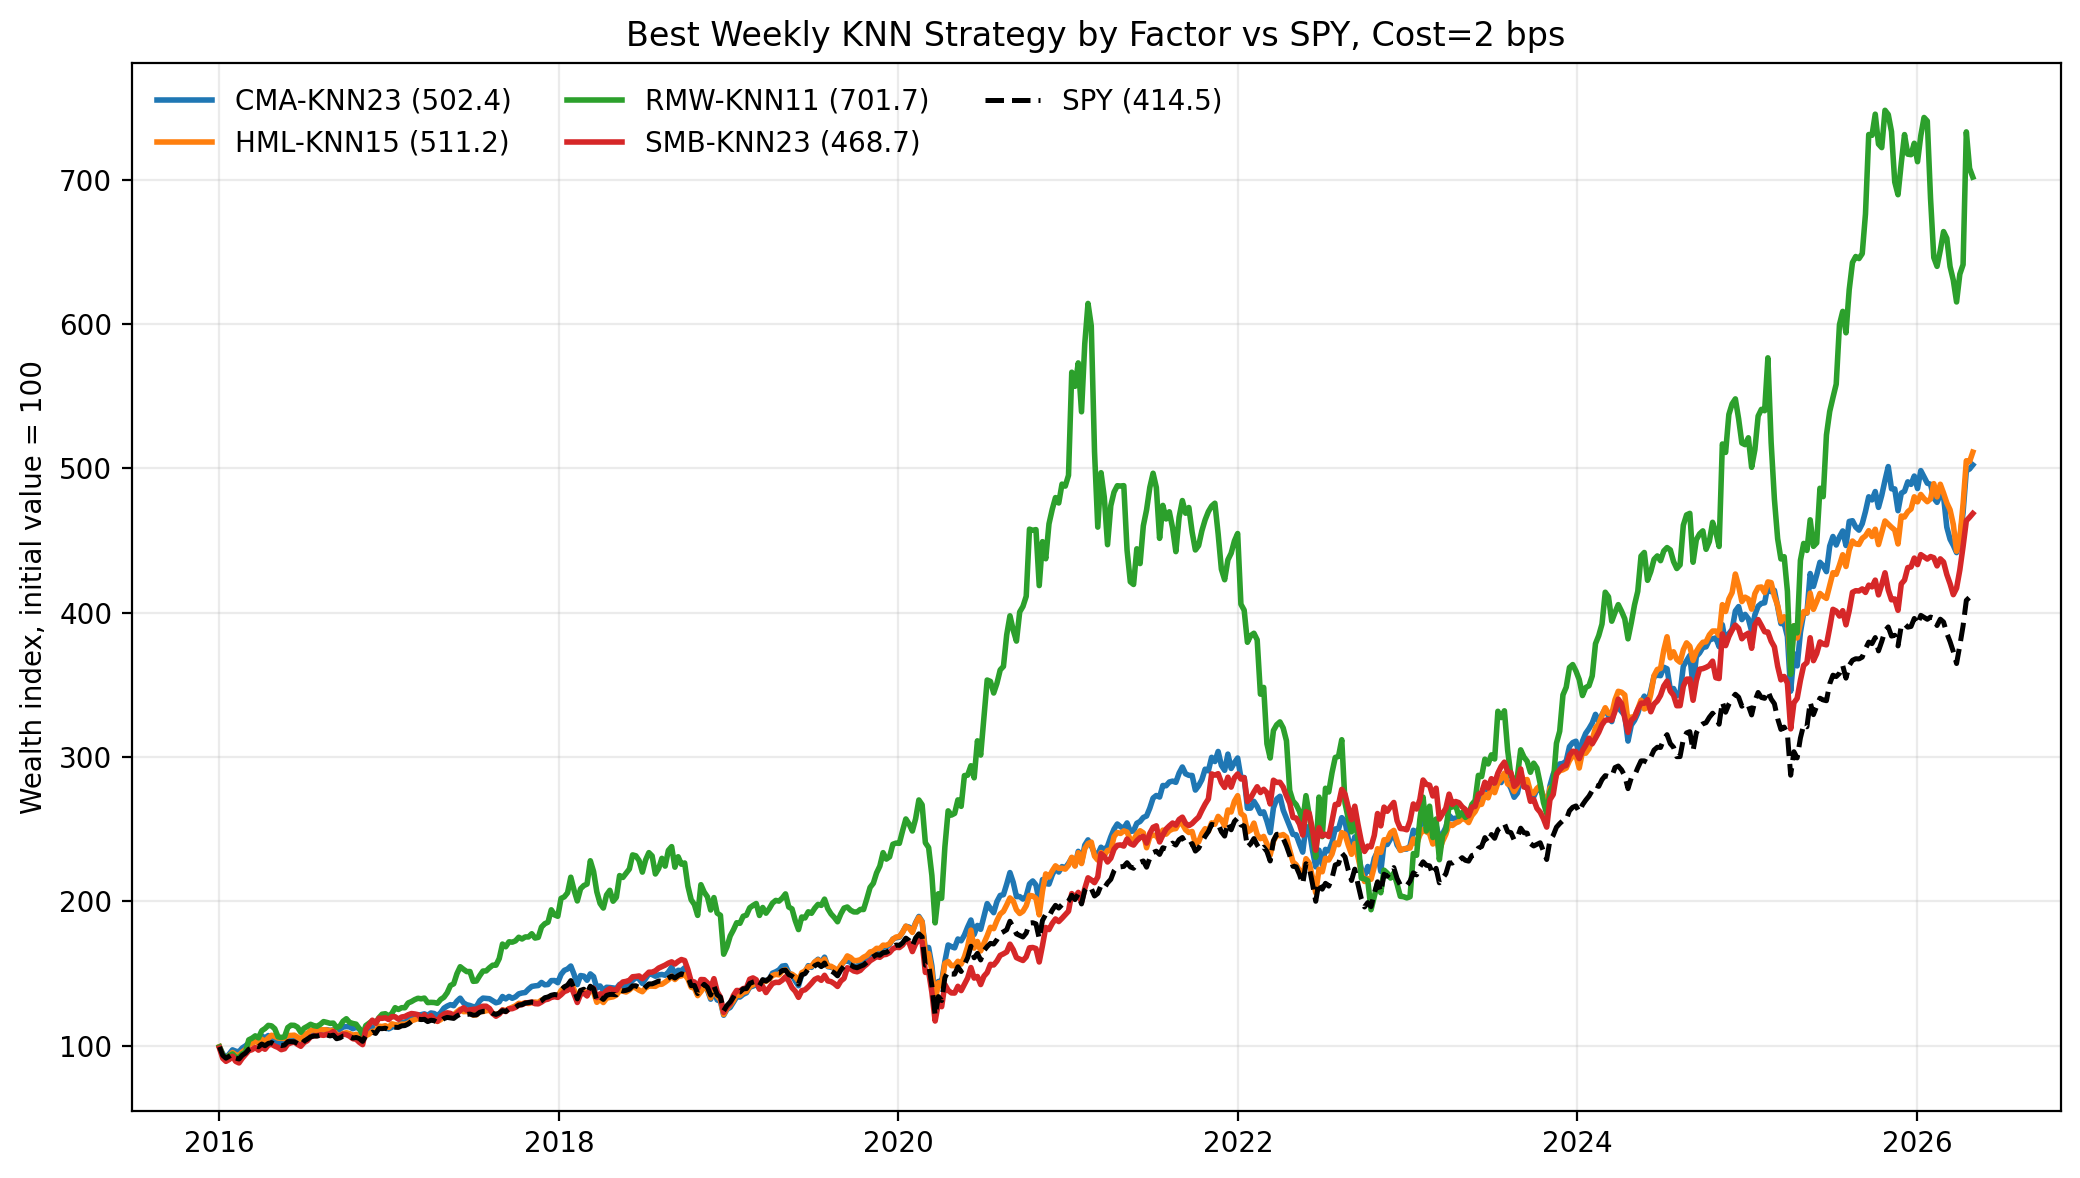
\includegraphics[width=\textwidth]{../outputs/paper_weekly_knn_primary_strategy_bps_2.png}
\caption{Best weekly KNN strategy by factor versus SPY at 2 bps per switch}
\label{fig:weekly_knn_bps2}
\end{figure}

Figure \ref{fig:weekly_logit_bps2} reports the corresponding 2 basis point results for weekly logistic regression. Logistic regression is less uniformly successful than KNN in the weekly specification. The CMA logit strategy remains above SPY, while HML, RMW, and SMB finish below SPY. This indicates that the interpretability of the linear classifier does not by itself guarantee stronger implementation performance.

\begin{figure}[H]
\centering
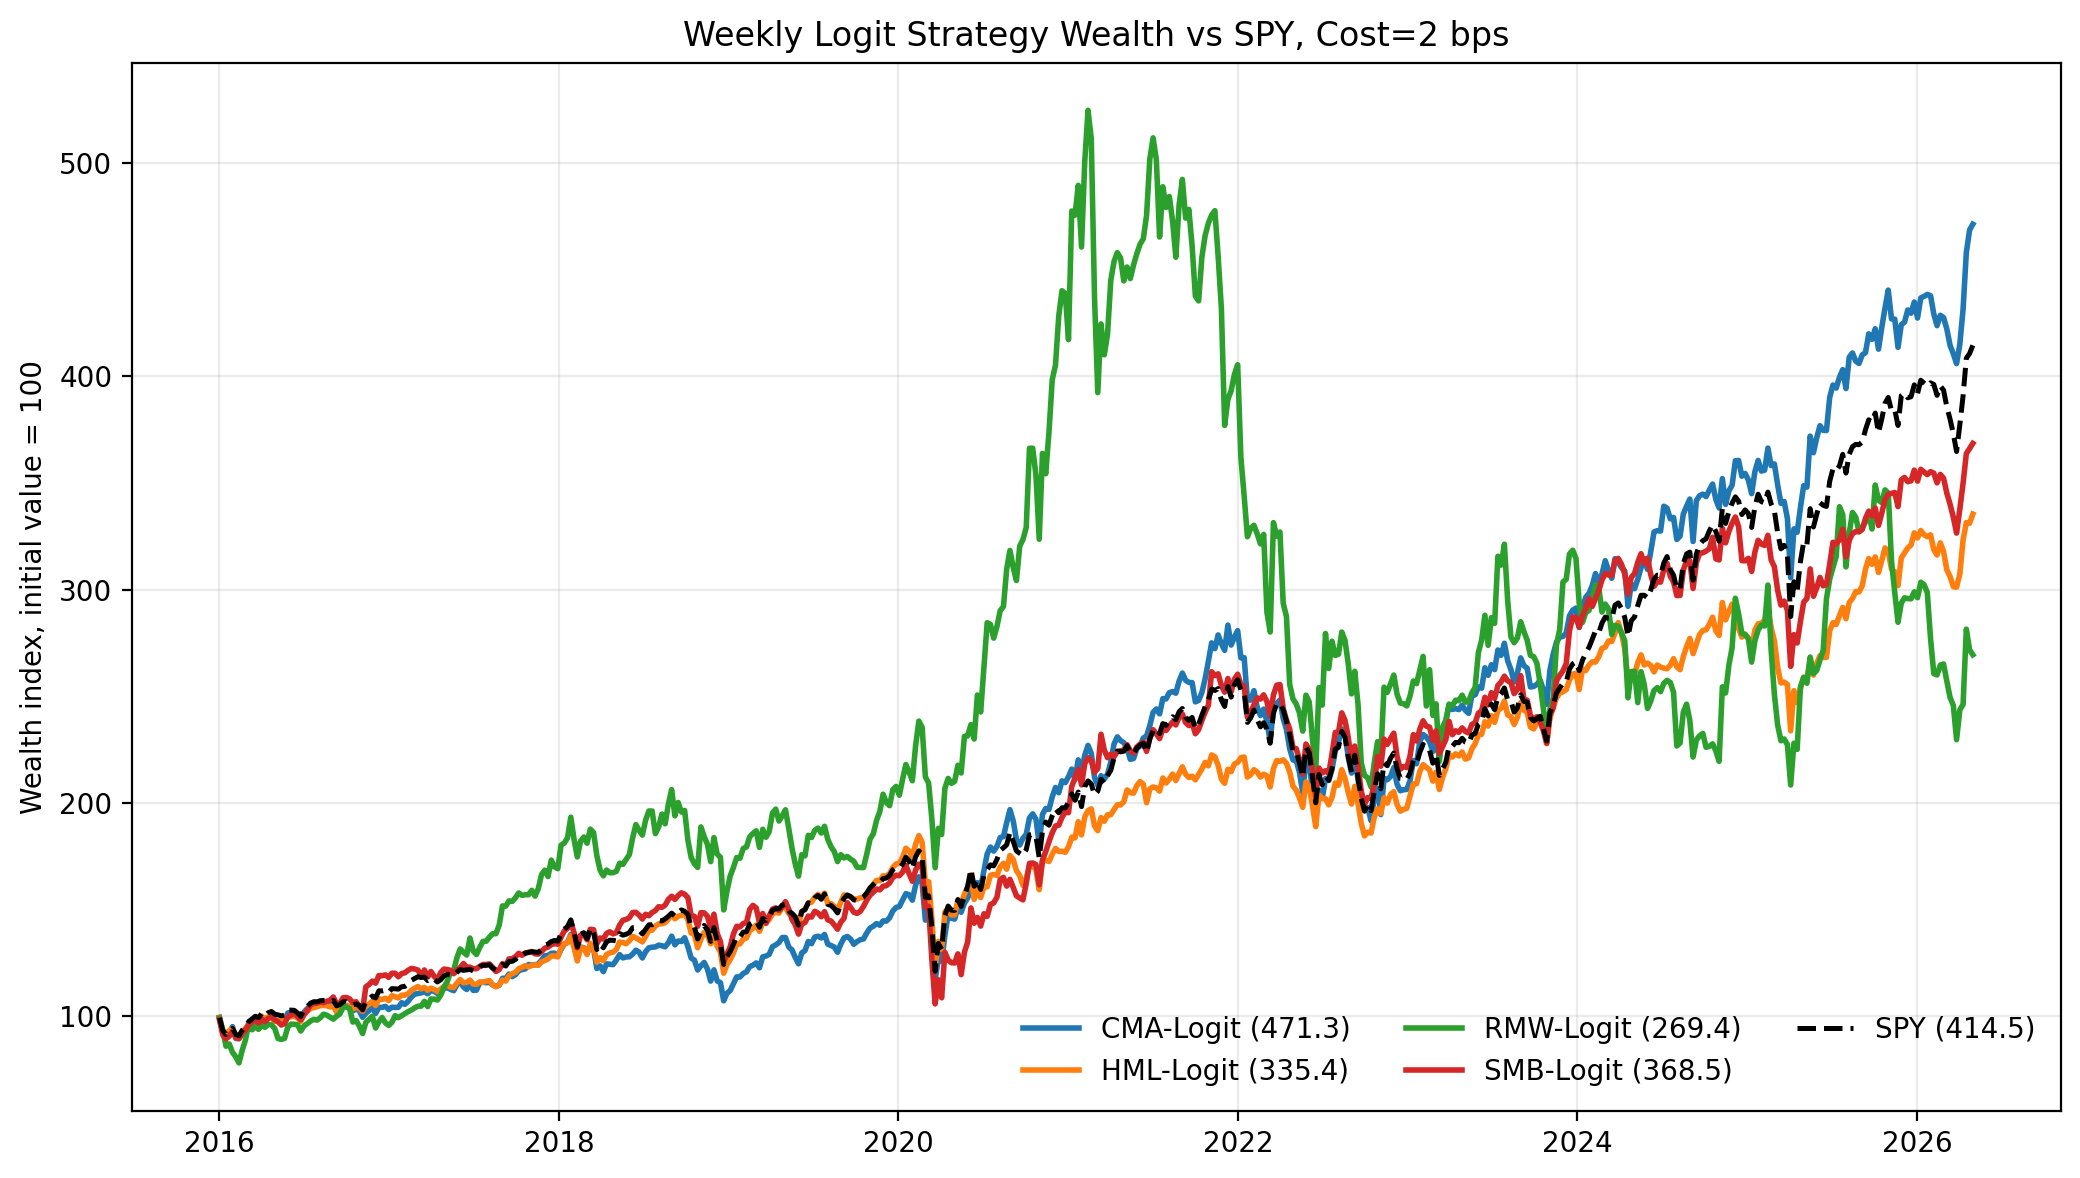
\includegraphics[width=\textwidth]{../outputs/paper_weekly_logit_primary_strategy_bps_2.png}
\caption{Weekly logistic strategy wealth versus SPY at 2 bps per switch}
\label{fig:weekly_logit_bps2}
\end{figure}

Figures \ref{fig:weekly_winners_bps2} and \ref{fig:weekly_losers_bps2} report the 2 basis point results for the rule based Winners and Losers strategies at \(k=13\). The rule based strategies are more factor-specific than KNN. Winners performs well for CMA and HML, while Losers performs well for CMA and RMW. This difference reinforces the point that short horizon continuation and reversal are not universal across ETF factor proxies.

\begin{figure}[H]
\centering
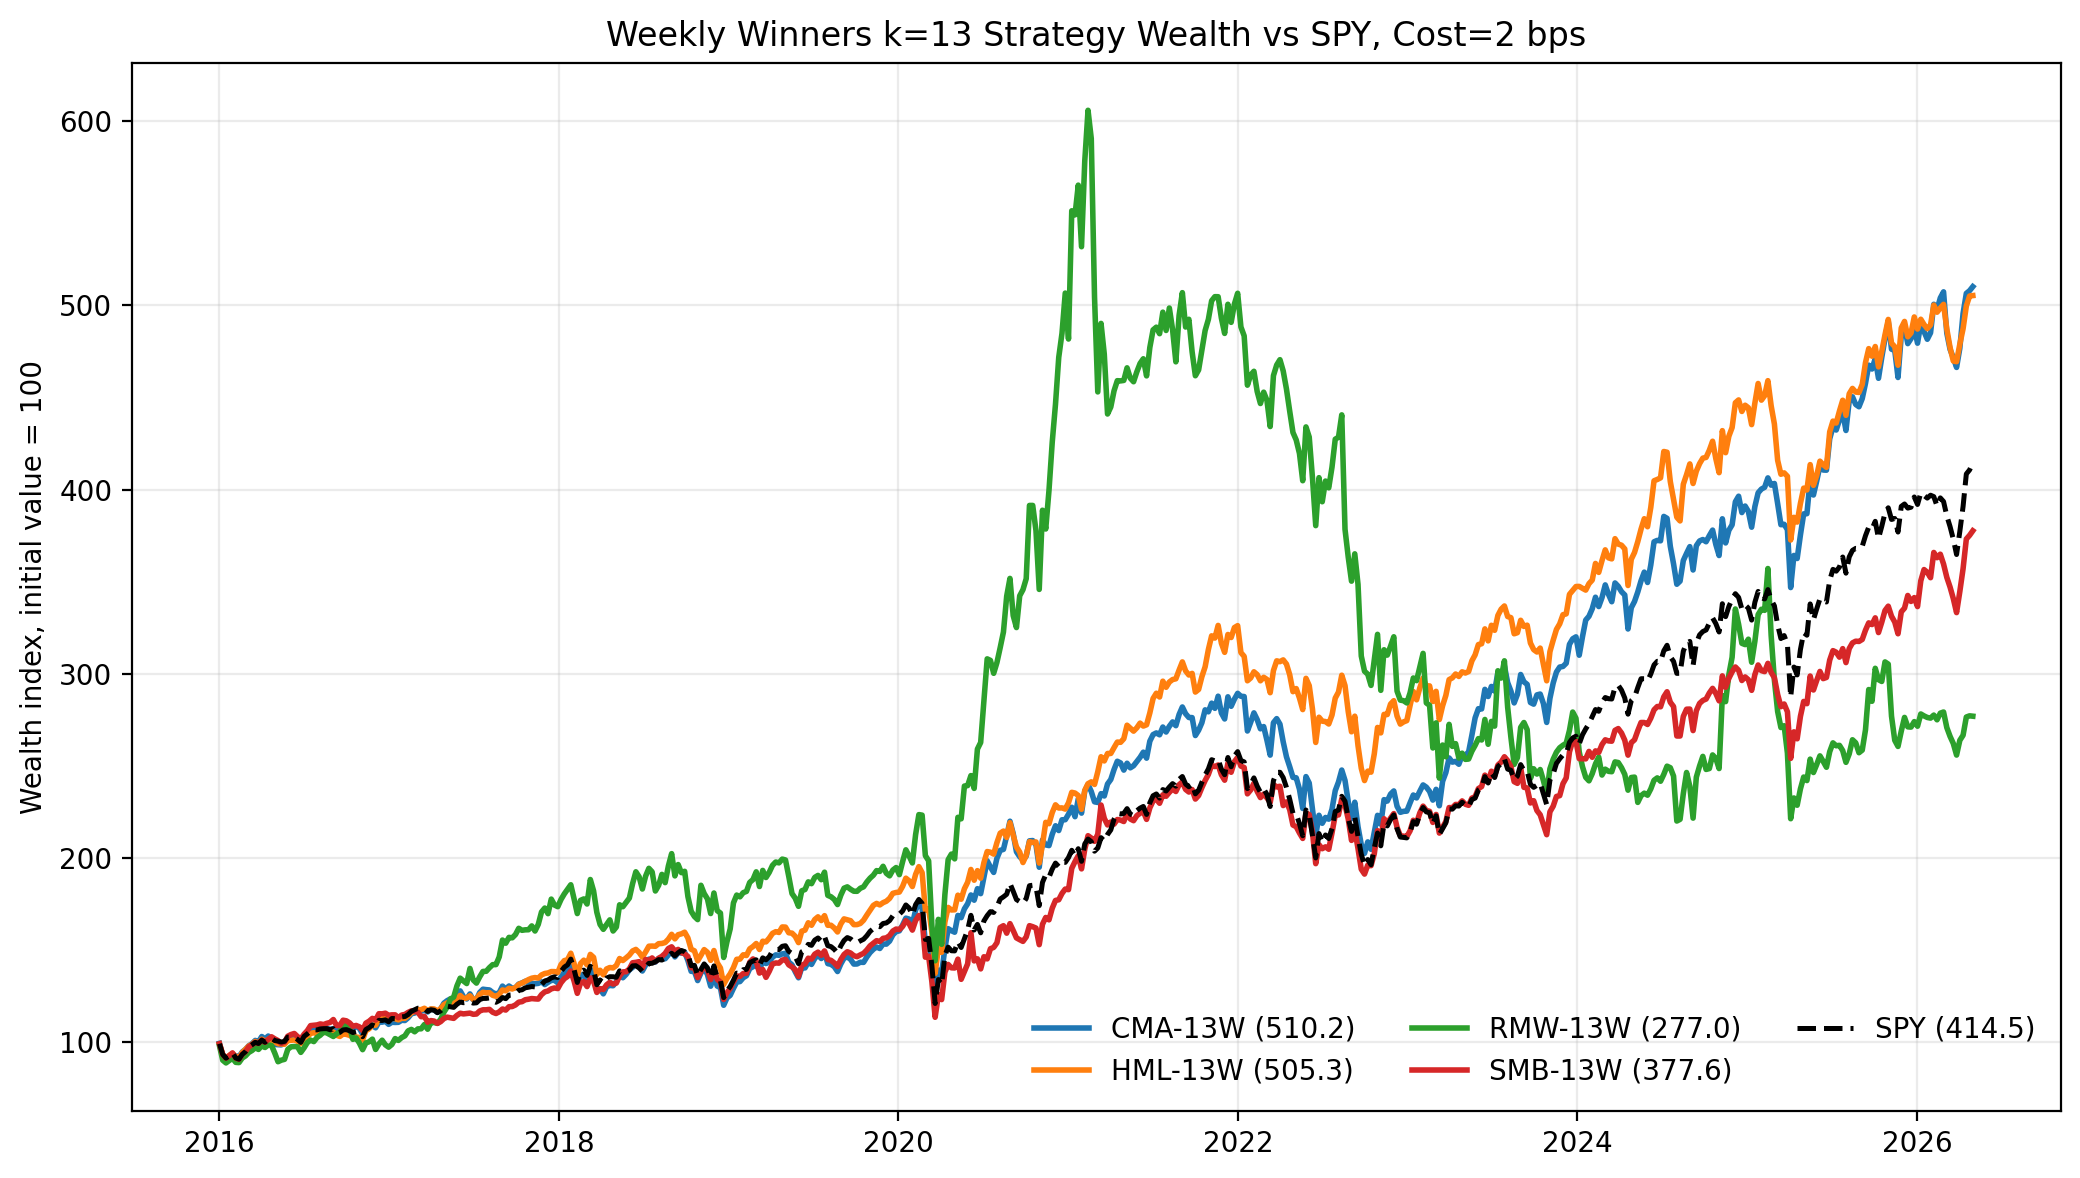
\includegraphics[width=\textwidth]{../outputs/paper_weekly_winners_k13_primary_strategy_bps_2.png}
\caption{Weekly Winners \(k=13\) strategy wealth versus SPY at 2 bps per switch}
\label{fig:weekly_winners_bps2}
\end{figure}

\begin{figure}[H]
\centering
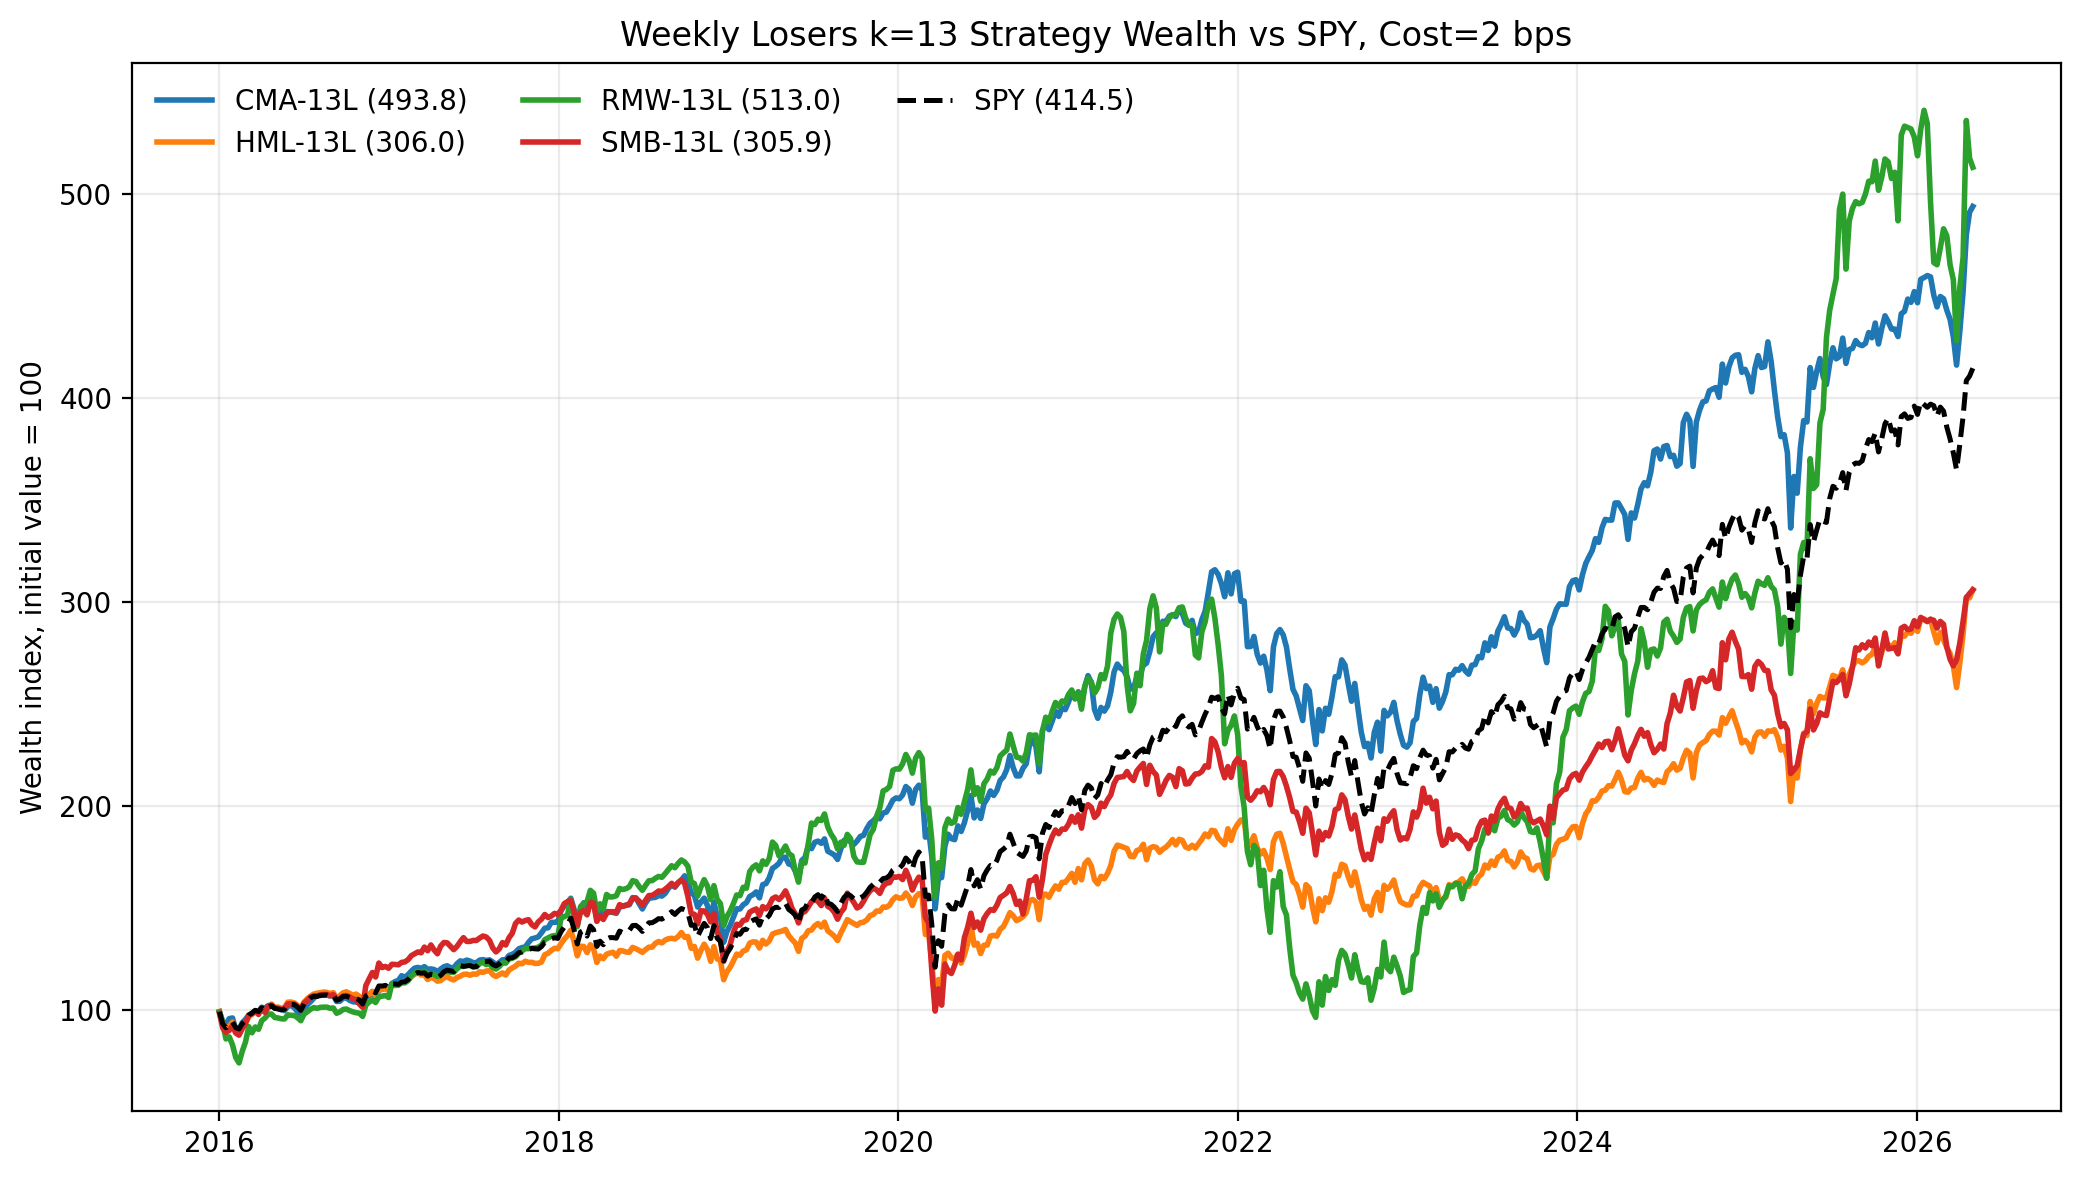
\includegraphics[width=\textwidth]{../outputs/paper_weekly_losers_k13_primary_strategy_bps_2.png}
\caption{Weekly Losers \(k=13\) strategy wealth versus SPY at 2 bps per switch}
\label{fig:weekly_losers_bps2}
\end{figure}

Weekly trading reduces the number of switches and often produces smoother risk adjusted performance. This is useful from an implementation perspective because daily classification models can appear profitable before costs but become fragile when turnover rises. The weekly KNN results make this point directly. Relative to the best daily KNN specification, the best weekly KNN specification reduces switches by approximately 82 percent for CMA, 75 percent for HML, 75 percent for RMW, and 83 percent for SMB. At the same time, the Sharpe ratio rises for CMA, HML, and SMB, and is essentially unchanged for RMW. This is a useful economic result because it shows that lowering the trading frequency does not merely reduce costs mechanically. It also appears to remove part of the short horizon noise in the classification problem.

The logistic regression results add a second diagnostic. Logistic regression is less flexible than KNN, but it is easier to interpret and generally trades less often. The daily HML logistic strategy is the strongest example: it produces a Sharpe ratio of 0.974, a final wealth of 583.3, and 469 switches. The best daily HML KNN strategy has a Sharpe ratio of 0.858, a final wealth of 456.9, and 853 switches. In this case, the more parsimonious classifier dominates the more flexible nearest neighbor rule. This matters for the paper because it weakens a purely data mining interpretation of the results. The strongest HML result does not require the most adaptive or highest turnover model.

The evidence does not imply that KNN universally dominates logistic regression or the rule based strategy. Rather, model ranking depends on the factor, the proxy, and the trading frequency.

\subsection{Out of Sample Evidence}

Table \ref{tab:oos_results} reports a rolling out of sample test for the rule based Winners and Losers family. For each factor and test year, the strategy is selected using the previous three full calendar years and then evaluated in the next year. This test is deliberately stricter than reporting the best full sample rule because the model choice must be made using only prior data. The KNN and logistic results are evaluated using expanding windows, but their model class is not reselected year by year in this table.

\begin{table}[H]
\centering
\caption{Out of sample strategy performance}
\label{tab:oos_results}
\scriptsize
\resizebox{0.95\textwidth}{!}{
\begin{tabular}{lrrrrrrrr}
\toprule
Factor & Obs. & Final & CAGR & Vol. & Sharpe & MDD & Switches & Acc. \\
\midrule
CMA & 2093 & 351.1 & 16.3\% & 22.0\% & 0.797 & -31.6\% & 327 & 49.7\% \\
HML & 2093 & 242.5 & 11.3\% & 19.9\% & 0.635 & -34.0\% & 275 & 50.0\% \\
RMW & 2093 & 290.2 & 13.7\% & 31.5\% & 0.565 & -50.2\% & 394 & 49.4\% \\
SMB & 2093 & 215.1 & 9.7\% & 21.8\% & 0.532 & -34.3\% & 307 & 49.7\% \\
\bottomrule
\end{tabular}}
\end{table}

The out of sample results are more restrained than the best full sample results. This is expected and is important for interpretation. The rolling procedure still produces positive terminal wealth for all four factors, but Sharpe ratios are lower and classification accuracy remains close to 50 percent. The value of the strategies, when present, comes from the payoff asymmetry of being on the right side during important periods, not from consistently high hit rates.

Two additional implementation diagnostics are reported in Appendix \ref{app:robustness}. The transaction cost sensitivity results show that performance weakens as costs increase, but weekly KNN specifications are less sensitive because they switch less frequently. The payoff asymmetry results show why strategies can generate positive economic performance even when classification accuracy is close to 50 percent: correct classifications tend to occur in higher payoff periods than the losses observed during incorrect classifications.

\section{Discussion}

The empirical results support three conclusions. First, ETF factor proxy construction must be validated before strategy results are interpreted. SMB and HML have the strongest ETF representations in this study, while RMW and CMA are more moderate. This means that the phrase factor timing should be used carefully. In some cases the strategy is timing a tradable ETF spread that only partially overlaps with the intended academic factor. The RMW and CMA proxies remain open to debate because QUAL, ARKK, SPHQ, and QQQ do not reproduce the original characteristic sorted construction of the Fama and French factors. They should therefore be interpreted as economically motivated ETF approximations, not exact factor replicating portfolios.

Second, weekly classification results are economically more plausible than many daily specifications. Daily models use more observations, but they also trade more frequently and are more exposed to microstructure noise, estimation instability, and transaction costs. Weekly trading sacrifices some responsiveness but reduces turnover. The weekly HML KNN result is particularly notable because it combines a reasonable proxy validation score, strong risk adjusted performance, and fewer switches than its daily counterpart. The broader weekly KNN pattern strengthens this point, since the reduction in switches is large across all four factors and does not come with a uniform loss in Sharpe ratios.

Third, the results caution against selecting a single best model from the full sample. The model rankings vary by factor. Logistic regression is strong for daily HML, while KNN is stronger for several weekly specifications. The Winners and Losers rule is attractive for some ETF pairs but weak for others. For a finance audience, this heterogeneity is a feature rather than a nuisance. It shows that implementable factor timing is conditional on the quality of the tradable proxy and the stability of the underlying relative return process. It also gives the empirical section a natural hierarchy: proxy validation comes first, trading performance comes second, and model complexity is evaluated only after turnover, transaction costs, payoff asymmetry, and out of sample behavior are considered.

The analysis also raises a standard multiple testing concern. Several values of \(k\), trading frequencies, and model classes are evaluated, so the strongest individual strategy should not be interpreted as a stand alone discovery. For this reason, the paper emphasizes patterns that survive across related diagnostics: whether the proxy has independent factor validation, whether the strategy remains viable after transaction costs, whether turnover is economically plausible, whether payoff asymmetry rather than hit rate alone explains performance, and whether rolling out of sample evidence points in the same direction. This interpretation is deliberately more conservative than selecting the highest terminal wealth from the full sample.

The main limitation of the study is the ETF sample length. Some ETFs used in the proxy set begin trading after the early 2000s, which restricts the common sample to the post 2014 period. This avoids look ahead bias and unequal sample comparisons, but it also means that the results are estimated over one market era. Future work could examine longer histories using stock level characteristic sorted portfolios or institutional factor replication data, then compare those results with ETF based implementation.

\section{Conclusion}

This paper studies whether liquid ETF pairs can serve as tradable proxies for the non market Fama and French factors and whether simple classification rules can improve allocation between the ETF legs. The answer is mixed in an economically informative way. ETF proxy quality is strong for SMB, meaningful for HML, and moderate for RMW and CMA. Strategy performance is also uneven. Some rules generate attractive performance after transaction costs, especially selected HML, RMW, and revised CMA classification strategies, but no method dominates across all factors and frequencies. The final classification tests add two practical lessons. First, weekly KNN can sharply reduce turnover while preserving much of the predictive content in the signals. Second, logistic regression can be competitive when the underlying proxy is economically coherent, as in the HML pair.

The broader implication is that implementable factor timing should be evaluated in two stages. First, the tradable proxy must be shown to capture the intended academic factor. Second, the timing rule must be tested after costs and with attention to turnover. Without the first step, high returns may simply reflect ETF specific behavior. Without the second, apparent predictability may not survive implementation. The results therefore support a cautious view: ETF based factor timing can be useful, but its credibility depends on proxy validation, conservative backtesting, and transparent treatment of trading frictions.

\appendix
\section{Implementation Robustness}
\label{app:robustness}

Table \ref{tab:cost_sensitivity} reports terminal wealth and Sharpe ratios for selected strategies at 0, 2, 5, and 10 basis points per switch. The strategies weaken as trading costs rise, as expected. The weekly KNN specifications are less sensitive because they trade less frequently.

\begin{table}[H]
\centering
\caption{Transaction cost sensitivity: final wealth and Sharpe ratio}
\label{tab:cost_sensitivity}
\scriptsize
\resizebox{\textwidth}{!}{
\begin{tabular}{lrrrr}
\toprule
Strategy & 0 bps & 2 bps & 5 bps & 10 bps \\
\midrule
Daily CMA Losers & 484.1 / 0.787 & 454.9 / 0.760 & 414.4 / 0.719 & 354.7 / 0.651 \\
Daily HML Logit & 640.7 / 1.021 & 583.3 / 0.974 & 506.8 / 0.904 & 400.8 / 0.787 \\
Weekly HML KNN & 533.4 / 1.006 & 511.2 / 0.983 & 479.6 / 0.948 & 431.3 / 0.889 \\
Weekly SMB KNN & 487.6 / 0.887 & 468.7 / 0.868 & 441.7 / 0.838 & 400.2 / 0.788 \\
\bottomrule
\end{tabular}}
\end{table}

Table \ref{tab:payoff_asymmetry} reports directional accuracy, payoff asymmetry, break-even accuracy, and the average timing contribution for selected strategies. For the selected strategies, correct classifications often occur in periods with larger absolute proxy spreads than incorrect classifications. This helps explain why strategies can have meaningful economic performance even when accuracy is only modestly above 50 percent.

\begin{table}[H]
\centering
\caption{Payoff asymmetry and directional accuracy in selected strategies}
\label{tab:payoff_asymmetry}
\scriptsize
\resizebox{\textwidth}{!}{
\begin{tabular}{lrrrrrr}
\toprule
Strategy & Accuracy & $\mu^{+}$ & $\mu^{-}$ & $p^{\ast}$ & Timing & PT Stat. (p) \\
\midrule
Daily CMA Losers (k = 13) & 50.6\% & 0.450\% & 0.476\% & 51.4\% & -0.39 & 1.06 (0.144) \\
Daily HML Logit & 53.1\% & 0.546\% & 0.536\% & 49.6\% & 1.90 & 2.05 (0.020) \\
Daily HML KNN15 & 51.9\% & 0.546\% & 0.536\% & 49.6\% & 1.25 & 1.05 (0.146) \\
Daily RMW KNN11 & 51.7\% & 1.400\% & 1.403\% & 50.1\% & 2.34 & 1.72 (0.042) \\
Daily CMA KNN3 & 50.5\% & 0.471\% & 0.468\% & 49.8\% & 0.33 & 0.26 (0.397) \\
Daily SMB KNN3 & 49.9\% & 0.586\% & 0.562\% & 48.9\% & 0.57 & -0.24 (0.593) \\
Weekly HML Winners (k = 13) & 52.3\% & 1.150\% & 1.106\% & 49.0\% & 3.70 & 0.81 (0.208) \\
Weekly CMA Losers (k = 13) & 50.4\% & 1.008\% & 1.018\% & 50.2\% & 0.22 & 0.51 (0.304) \\
Weekly CMA KNN23 & 48.3\% & 1.060\% & 0.970\% & 47.8\% & 0.61 & -1.36 (0.913) \\
Weekly HML KNN15 & 52.0\% & 1.231\% & 1.111\% & 47.4\% & 5.38 & 0.68 (0.249) \\
Weekly RMW KNN11 & 53.0\% & 3.114\% & 2.991\% & 49.0\% & 12.25 & 1.17 (0.122) \\
Weekly SMB KNN23 & 52.4\% & 1.297\% & 1.163\% & 47.3\% & 6.32 & 1.06 (0.144) \\
\bottomrule
\end{tabular}}
\begin{flushleft}
\footnotesize{\textit{Notes:} $\mu^{+}$ and $\mu^{-}$ are the average absolute ETF proxy spreads $|F^{ETF}_{j,t}|$ in correctly and incorrectly classified periods. $p^{\ast}=\mu^{-}/(\mu^{+}+\mu^{-})$ is the break-even accuracy. Timing is the average gross timing component $\frac{1}{2}d_{j,t}F^{ETF}_{j,t}$, in basis points per day or per week. PT Stat. is the Pesaran and Timmermann directional statistic with its one-sided p-value. All strategy returns are net of 2 basis points per switch, while the timing component is shown before costs.}
\end{flushleft}
\end{table}

\authorcontributions{Conceptualization, S.B. and E.P.; methodology, S.B.; software, S.B.; data curation, S.B.; formal analysis, S.B. and E.P.; visualization, S.B.; writing, original draft preparation, S.B.; writing, review and editing, S.B. and E.P.; supervision, E.P. All authors have read and agreed to the published version of the manuscript.}

\funding{This research received no external funding.}

\dataavailability{The Fama and French factor data are available from the Kenneth R. French Data Library. ETF return data and replication code are available from the authors upon reasonable request.}

\acknowledgments{The authors thank the Department of Computer Science at Boston University Metropolitan College for support.}

\conflictsofinterest{The authors declare no conflict of interest.}

\printendnotes[custom]

\reftitle{References}
\bibliography{citations}

\end{document}
